% Capitolul 7: Cointegrare și Modele VECM
% Prezentare academică de calitate Harvard
% Program de licență, Academia de Studii Economice din București

\documentclass[9pt, aspectratio=169, t]{beamer}

% Asigură încadrarea conținutului pe diapozitive
\setbeamersize{text margin left=8mm, text margin right=8mm}

%=============================================================================
% CONFIGURARE TEMĂ ȘI STIL
%=============================================================================
\usetheme{default}
% Using default theme for clean header/footer control

% Color Palette (matching Redispatch PDF)
\definecolor{MainBlue}{RGB}{26, 58, 110}
\definecolor{AccentBlue}{RGB}{26, 58, 110}
\definecolor{IDAred}{RGB}{205, 0, 0}
\definecolor{DarkGray}{RGB}{51, 51, 51}
\definecolor{MediumGray}{RGB}{128, 128, 128}
\definecolor{LightGray}{RGB}{248, 248, 248}
\definecolor{VeryLightGray}{RGB}{235, 235, 235}
\definecolor{KeynoteGray}{RGB}{218, 218, 218}
\definecolor{SectionGray}{RGB}{120, 120, 120}
\definecolor{FooterGray}{RGB}{100, 100, 100}
\definecolor{Crimson}{RGB}{220, 53, 69}
\definecolor{Forest}{RGB}{46, 125, 50}
\definecolor{Amber}{RGB}{181, 133, 63}
\definecolor{Orange}{RGB}{230, 126, 34}
\definecolor{Purple}{RGB}{142, 68, 173}

% Gradient background (exact Keynote 315° gradient: white to RGB 218,218,218)
\setbeamertemplate{background}{%
    \begin{tikzpicture}[remember picture, overlay]
        \shade[shading=axis, shading angle=315,
        top color=white, bottom color=KeynoteGray]
        (current page.south west) rectangle (current page.north east);
    \end{tikzpicture}%
}
% Fallback solid color for compatibility
\setbeamercolor{background canvas}{bg=}

\setbeamercolor{palette primary}{bg=MainBlue, fg=white}
\setbeamercolor{palette secondary}{bg=MainBlue!85, fg=white}
\setbeamercolor{palette tertiary}{bg=MainBlue!70, fg=white}
\setbeamercolor{structure}{fg=MainBlue}
\setbeamercolor{title}{fg=IDAred}
\setbeamercolor{frametitle}{fg=IDAred, bg=}
\setbeamercolor{block title}{bg=MainBlue, fg=white}
\setbeamercolor{block body}{bg=VeryLightGray, fg=DarkGray}
\setbeamercolor{block title alerted}{bg=Crimson, fg=white}
\setbeamercolor{block body alerted}{bg=Crimson!8, fg=DarkGray}
\setbeamercolor{block title example}{bg=Forest, fg=white}
\setbeamercolor{block body example}{bg=Forest!8, fg=DarkGray}
\setbeamercolor{item}{fg=MainBlue}

% Footer colors (override Madrid theme blue)
\setbeamercolor{author in head/foot}{fg=FooterGray, bg=}
\setbeamercolor{title in head/foot}{fg=FooterGray, bg=}
\setbeamercolor{date in head/foot}{fg=FooterGray, bg=}
\setbeamercolor{section in head/foot}{fg=FooterGray, bg=}
\setbeamercolor{subsection in head/foot}{fg=FooterGray, bg=}

% Bullet styles (apply everywhere including blocks)
\setbeamertemplate{itemize item}{\color{MainBlue}$\boxdot$}
\setbeamertemplate{itemize subitem}{\color{MainBlue}$\blacktriangleright$}
\setbeamertemplate{itemize subsubitem}{\color{MainBlue}\tiny$\bullet$}
\setbeamertemplate{itemize/enumerate body begin}{\normalsize}
\setbeamertemplate{itemize/enumerate subbody begin}{\normalsize}

% Item spacing - compact style
\setlength{\leftmargini}{10pt}       % Level 1: minimal indent
\setlength{\leftmarginii}{10pt}      % Level 2: minimal additional indent

\setbeamertemplate{navigation symbols}{}

%=============================================================================
% CUSTOM HEADLINE
%=============================================================================
\setbeamertemplate{headline}{%
    \vskip10pt%
    \hbox to \paperwidth{%
        \hskip0.5cm%
        {\small\color{FooterGray}\renewcommand{\hyperlink}[2]{##2}\insertsectionhead}%
        \hfill%
        \textcolor{FooterGray}{\small\insertframenumber}%
        \hskip0.5cm%
    }%
    \vskip4pt%
    {\color{FooterGray}\hrule height 0.4pt}%
}

%=============================================================================
% CUSTOM FOOTER
%=============================================================================
\usepackage{fontawesome5}

\setbeamertemplate{footline}{%
    {\color{FooterGray}\hrule height 0.4pt}%
    \vskip4pt%
    \hbox to \paperwidth{%
        \hskip0.5cm%
        \textcolor{FooterGray}{\small Analiza și Prognoza seriilor de timp}%
        \hfill%
        \raisebox{-0.1em}{%
            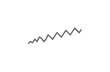
\begin{tikzpicture}[x=0.08em, y=0.08em, line width=0.4pt]
                \draw[FooterGray] (0,3) -- (1,4) -- (2,3.5) -- (3,5) -- (4,4) -- (5,6) -- (6,5.5) -- (7,4) -- (8,5) -- (9,7) -- (10,6) -- (11,5) -- (12,6.5) -- (13,8) -- (14,7) -- (15,6) -- (16,7.5) -- (17,9) -- (18,8) -- (19,7) -- (20,8.5) -- (21,10) -- (22,9) -- (23,8) -- (24,9.5);
            \end{tikzpicture}%
        }%
        \hskip0.5cm%
    }%
    \vskip6pt%
}

%=============================================================================
% PACHETE
%=============================================================================
\usepackage[utf8]{inputenc}
\usepackage[T1]{fontenc}
\usepackage{amsmath, amssymb, amsthm}
\usepackage{mathtools}
\usepackage{bm}
\usepackage{tikz}
\usetikzlibrary{arrows.meta, positioning, shapes, calc, decorations.pathreplacing, shadings}
\usepackage{booktabs}
\usepackage{multirow}
\usepackage{array}
\usepackage{graphicx}
\usepackage{hyperref}
\usepackage{colortbl}
\hypersetup{colorlinks=true, linkcolor=MainBlue, urlcolor=MainBlue}
\graphicspath{{../../logos/}{../../charts/}}
\hfuzz=2pt  % Suppress tiny overfull warnings (<2pt)

%=============================================================================
%=============================================================================
% Usage: \quantlet{QuantletName}{https://github.com/...}
\newcommand{\quantlet}[2]{%
    \hfill\href{#2}{\raisebox{-0.15em}{\includegraphics[height=0.7em]{ql_logo.png}}\textcolor{MainBlue}{\tiny\ #1}}%
}


%=============================================================================
% MEDII PENTRU TEOREME
%=============================================================================
\theoremstyle{definition}
\setbeamertemplate{theorems}[numbered]
\newtheorem{defn}{Definiție}
\newtheorem{thm}{Teoremă}
\newtheorem{prop}{Propoziție}
\newtheorem{rmk}{Observație}

%=============================================================================
% COMENZI PERSONALIZATE
%=============================================================================
\newcommand{\E}{\mathbb{E}}
\newcommand{\Var}{\text{Var}}
\newcommand{\Cov}{\text{Cov}}
\newcommand{\Corr}{\text{Corr}}
\newcommand{\R}{\mathbb{R}}
\newcommand{\N}{\mathbb{N}}
\newcommand{\Z}{\mathbb{Z}}
\newcommand{\RMSE}{\text{RMSE}}
\newcommand{\MAE}{\text{MAE}}
\newcommand{\MAPE}{\text{MAPE}}
\newcommand{\bY}{\mathbf{Y}}
\newcommand{\bA}{\mathbf{A}}
\newcommand{\bSigma}{\boldsymbol{\Sigma}}
\newcommand{\bPhi}{\boldsymbol{\Phi}}
\newcommand{\bGamma}{\boldsymbol{\Gamma}}
\newcommand{\bPi}{\boldsymbol{\Pi}}
\newcommand{\bc}{\mathbf{c}}
\newcommand{\balpha}{\boldsymbol{\alpha}}
\newcommand{\bbeta}{\boldsymbol{\beta}}
\newcommand{\bepsilon}{\boldsymbol{\varepsilon}}

%=============================================================================
% PAGINĂ TITLU PERSONALIZATĂ
%=============================================================================
\defbeamertemplate*{title page}{hybrid}[1][]
{
    \vspace{0.2cm}
    % Logos row - top header (with clickable links)
    \begin{center}
        \href{https://www.ase.ro}{\includegraphics[height=1.0cm]{ase_logo.png}}\hspace{0.3cm}%
        \href{https://theida.net}{\includegraphics[height=1.0cm]{ida_logo.png}}\hspace{0.3cm}%
        \href{https://blockchain-research-center.com}{\includegraphics[height=1.0cm]{brc_logo.png}}\hspace{0.3cm}%
        \href{https://www.ai4efin.ase.ro}{\includegraphics[height=1.0cm]{ai4efin_logo.png}}\hspace{0.3cm}%
        \href{https://ipe.ro/new}{\includegraphics[height=1.0cm]{acad_logo.png}}\hspace{0.3cm}%
        \href{https://www.digital-finance-msca.com}{\includegraphics[height=1.0cm]{msca_logo.png}}%
    \end{center}

    \vspace{0.6cm}

    % Main title with Q logos on sides (with clickable links)
    \begin{center}
        \begin{minipage}{0.1\textwidth}
            \centering
            \href{https://quantlet.com}{\includegraphics[height=1.1cm]{ql_logo.png}}
        \end{minipage}%
        \begin{minipage}{0.78\textwidth}
            \centering
            {\LARGE\bfseries\usebeamercolor[fg]{title}\inserttitle}

            \vspace{0.3cm}

            {\usebeamerfont{subtitle}\usebeamercolor[fg]{title}\insertsubtitle}
        \end{minipage}%
        \begin{minipage}{0.1\textwidth}
            \centering
            \href{https://quantinar.com}{\includegraphics[height=1.1cm]{qr_logo.png}}
        \end{minipage}
    \end{center}

    \vspace{0.6cm}

    % Authors (left aligned)
    \hspace{0.5cm}{\usebeamerfont{author}\insertauthor}

    \vspace{0.3cm}

    % Institute/Affiliations (left aligned)
    \hspace{0.5cm}\begin{minipage}[t]{0.9\textwidth}
        \raggedright\small\insertinstitute
    \end{minipage}
}

%=============================================================================
% INFORMAȚII TITLU
%=============================================================================
\title[Analiza Seriilor de Timp]{Analiza și Prognoza seriilor de timp}
\subtitle{Capitolul 7: Cointegrare și Modele VECM}
\author[D.T. Pele]{Daniel Traian PELE}
\institute{Academia de Studii Economice din București\\
IDA Institute Digital Assets\\
Blockchain Research Center\\
AI4EFin Artificial Intelligence for Energy Finance\\
Academia Română, Institutul de Prognoză Economică\\
MSCA Digital Finance}
\date{}

\begin{document}

% Title page (no header/footer)
{
\setbeamertemplate{headline}{}
\setbeamertemplate{footline}{}
\begin{frame}
    \titlepage
\end{frame}
}

%=============================================================================
% OUTLINE
%=============================================================================
\begin{frame}{Cuprins}
    \vspace{-0.3cm}
    {\small
    \begin{columns}[T]
        \begin{column}{0.48\textwidth}
            \tableofcontents[sections={1-4}, hideallsubsections]
        \end{column}
        \begin{column}{0.48\textwidth}
            \tableofcontents[sections={5-8}, hideallsubsections]
        \end{column}
    \end{columns}
    }
\end{frame}

%=============================================================================
% LEARNING OBJECTIVES
%=============================================================================
\begin{frame}{Obiective de învățare}
    \begin{block}{La finalul acestui capitol, veți fi capabili să:}
        \begin{enumerate}
            \item Înțelegeți conceptul de \textbf{cointegrare} și relații de echilibru pe termen lung
            \item Recunoașteți și evitați problema \textbf{regresiei false}
            \item Aplicați metoda \textbf{Engle-Granger} în doi pași
            \item Efectuați testul \textbf{Johansen} pentru cointegrare multiplă
            \item Estimați și interpretați modele \textbf{VECM}
            \item Analizați viteza de ajustare și vectori de cointegrare
            \item Implementați analiza de cointegrare în \textbf{Python}
        \end{enumerate}
    \end{block}
\end{frame}

%=============================================================================
\section{Motivație}
%=============================================================================

\begin{frame}{De ce contează cointegrarea?}
    \begin{block}{Provocarea}
        \begin{itemize}
            \item Multe serii de timp economice/financiare sunt \textbf{nestaționare} (I(1))
            \item PIB, prețuri acțiuni, cursuri valutare, rate ale dobânzii au rădăcini unitare
            \item Regresia standard cu variabile I(1) $\Rightarrow$ \textbf{rezultate false}
            \item Diferențierea elimină nestaționaritatea dar pierde \textbf{informația pe termen lung}
        \end{itemize}
    \end{block}

    \vspace{0.2cm}

    \begin{alertblock}{Soluția: Cointegrarea}
        Unele serii nestaționare au un \textbf{trend stochastic comun}---se mișcă împreună pe termen lung. Această relație pe termen lung poate fi modelată!
    \end{alertblock}

    \vspace{0.2cm}

    \begin{exampleblock}{Premiul Nobel 2003}
        Clive Granger a primit Premiul Nobel în Economie (împreună cu Robert Engle) pentru dezvoltarea analizei de cointegrare---``metode pentru analiza seriilor de timp economice cu tendințe comune.''
    \end{exampleblock}
\end{frame}

\begin{frame}{Aplicații practice}
    \vspace{-0.2cm}
    {\small
    \begin{block}{Finanțe}
        \begin{itemize}\setlength{\itemsep}{0pt}
            \item \textbf{Pairs Trading}: Tranzacționarea spread-ului între acțiuni cointegrate
            \item \textbf{Structura pe Termene}: Rate dobânzi pe termen scurt și lung
            \item \textbf{Spot-Futures}: Relații de arbitraj
        \end{itemize}
    \end{block}

    \vspace{-0.05cm}

    \begin{block}{Macroeconomie}
        \begin{itemize}\setlength{\itemsep}{0pt}
            \item \textbf{Consum și Venit}: Ipoteza venitului permanent
            \item \textbf{Bani și Prețuri}: Teoria cantitativă a banilor
            \item \textbf{PPP}: Cursuri valutare și niveluri de prețuri
        \end{itemize}
    \end{block}

    \vspace{-0.05cm}

    \begin{block}{Analiza Politicilor}
        \begin{itemize}\setlength{\itemsep}{0pt}
            \item \textbf{Politica Fiscală}: Cheltuieli guvernamentale și venituri fiscale
            \item \textbf{Politica Monetară}: Transmiterea ratelor dobânzii
            \item \textbf{Piața Muncii}: Salarii și productivitate
        \end{itemize}
    \end{block}
    }
\end{frame}

%=============================================================================
\section{Regresia Falsă}
%=============================================================================

\begin{frame}{Problema regresiei false}
    \begin{block}{Granger \& Newbold (1974)}
        Regresarea unui mers aleatoriu pe un alt mers aleatoriu \textbf{independent}:
        $$Y_t = \alpha + \beta X_t + u_t$$
        unde $Y_t$ și $X_t$ sunt procese I(1) independente.
    \end{block}

    \vspace{0.1cm}

    \begin{alertblock}{Simptomele regresiei false}
        \begin{itemize}\setlength{\itemsep}{0pt}
            \item $R^2$ ridicat (adesea $> 0.9$) chiar dacă variabilele sunt \textbf{necorelate}!
            \item Statistici $t$ foarte semnificative (respingem $H_0: \beta = 0$)
            \item Statistica Durbin-Watson foarte mică ($DW \approx 0$)
            \item Reziduurile sunt nestaționare (au rădăcină unitară)
        \end{itemize}
    \end{alertblock}

    \vspace{0.05cm}

    {\footnotesize
    \begin{exampleblock}{Regulă Practică (Granger)}
        Dacă $R^2 > DW$, suspectați regresie falsă!
    \end{exampleblock}
    }
\end{frame}

\begin{frame}{Regresia falsă: exemplu vizual}
    \begin{center}
        \includegraphics[width=0.95\textwidth]{spurious_regression.pdf}
    \end{center}

    \vspace{0.1cm}

    {\footnotesize
    \textbf{Atenție}: Două mersuri aleatorii complet independente prezintă corelație ridicată ($R^2 > 0.8$) doar din întâmplare! De aceea avem nevoie de analiza cointegrării.
    }
    \quantlet{TSA\_charts/spurious\_regression}{https://github.com/QuantLet/TSA/tree/main/TSA_spurious_regression}
\end{frame}

%=============================================================================
\section{Conceptul de Cointegrare}
%=============================================================================

\begin{frame}{Definiția cointegrării}
    \begin{defn}[Cointegrare (Engle \& Granger, 1987)]
        Variabilele $Y_{1t}, Y_{2t}, \ldots, Y_{kt}$ sunt \textbf{cointegrate de ordinul $(d,b)$}, notat $CI(d,b)$, dacă:
        \begin{enumerate}
            \item Toate variabilele sunt integrate de ordinul $d$: $Y_{it} \sim I(d)$
            \item Există o combinație liniară $\bbeta' \bY_t = \beta_1 Y_{1t} + \cdots + \beta_k Y_{kt}$ care este integrată de ordinul $(d-b)$, unde $b > 0$
        \end{enumerate}
    \end{defn}

    \vspace{0.3cm}

    \begin{block}{Cazul Cel Mai Comun: $CI(1,1)$}
        \begin{itemize}
            \item Variabilele sunt $I(1)$ (au rădăcini unitare)
            \item Combinația liniară este $I(0)$ (staționară)
            \item Vectorul $\bbeta = (\beta_1, \ldots, \beta_k)'$ este \textbf{vectorul de cointegrare}
        \end{itemize}
    \end{block}

    \vspace{0.2cm}

    {\footnotesize
    Vectorul de cointegrare este unic doar până la înmulțire scalară. De obicei se normalizează: $\beta_1 = 1$.
    }
\end{frame}

\begin{frame}{Cointegrarea: exemplu vizual}
    \begin{center}
        \includegraphics[width=0.95\textwidth]{cointegrated_series.pdf}
    \end{center}

    \vspace{0.1cm}

    {\footnotesize
    \textbf{Ideea cheie}: Ambele serii sunt I(1) și evoluează împreună, dar combinația lor liniară (spread-ul) este staționară---aceasta este cointegrarea!
    }
    \quantlet{TSA\_charts/cointegrated\_series}{https://github.com/QuantLet/TSA/tree/main/TSA_cointegrated_series}
\end{frame}

\begin{frame}{Intuiție: tendințe stocastice comune}
    \vspace{-0.2cm}
    {\small
    \begin{block}{De ce Apare Cointegrarea?}
        Variabilele cointegrate împart \textbf{tendințe stocastice comune}:
        $$Y_{1t} = \gamma_1 \tau_t + S_{1t}, \qquad Y_{2t} = \gamma_2 \tau_t + S_{2t}$$
        unde $\tau_t$ este un mers aleatoriu comun și $S_{it}$ sunt componente staționare.
    \end{block}

    \vspace{-0.05cm}

    \begin{exampleblock}{Combinația Liniară Elimină Tendința}
        $$\gamma_2 Y_{1t} - \gamma_1 Y_{2t} = \gamma_2 S_{1t} - \gamma_1 S_{2t} \sim I(0)$$
    \end{exampleblock}

    \vspace{-0.05cm}

    \begin{alertblock}{Interpretare Economică}
        \begin{itemize}\setlength{\itemsep}{0pt}
            \item Cointegrarea reprezintă o \textbf{relație de echilibru pe termen lung}
            \item Variabilele pot devia pe termen scurt
            \item Dar sunt ``trase înapoi'' spre echilibru în timp
            \item Vectorul de cointegrare definește echilibrul
        \end{itemize}
    \end{alertblock}
    }
\end{frame}

\begin{frame}{Rangul de cointegrare}
    \begin{block}{Câte Relații de Cointegrare?}
        Pentru $k$ variabile care sunt $I(1)$:
        \begin{itemize}\setlength{\itemsep}{0pt}
            \item Maximum relații de cointegrare posibile: $r = k - 1$
            \item Dacă $r = 0$: Nu există cointegrare (variabilele divergează)
            \item Dacă $r = k$: Toate variabilele sunt $I(0)$ (contradicție)
        \end{itemize}
    \end{block}

    \vspace{0.1cm}

    \begin{exampleblock}{Exemplu: 3 Variabile}
        \begin{itemize}\setlength{\itemsep}{0pt}
            \item $r = 0$: Nu există cointegrare
            \item $r = 1$: O relație de cointegrare
            \item $r = 2$: Două relații de cointegrare (doar 1 tendință comună)
        \end{itemize}
    \end{exampleblock}

    \vspace{0.05cm}

    {\footnotesize
    Numărul de tendințe stocastice comune = $k - r$
    }
\end{frame}

%=============================================================================
\section{Metoda Engle-Granger}
%=============================================================================

\begin{frame}{Metoda în doi pași Engle-Granger}
    \vspace{-0.2cm}
    {\footnotesize
    \begin{block}{Pasul 1: Estimarea Regresiei de Cointegrare}
        Rulați regresia OLS (presupunând că $Y_t$ este variabila dependentă):
        $$Y_t = \alpha + \beta X_t + e_t$$
        Salvați reziduurile: $\hat{e}_t = Y_t - \hat{\alpha} - \hat{\beta} X_t$
    \end{block}

    \vspace{-0.05cm}

    \begin{block}{Pasul 2: Testarea Staționarității Reziduurilor}
        Testați dacă $\hat{e}_t$ este $I(0)$ folosind testul ADF:
        $$\Delta \hat{e}_t = \rho \hat{e}_{t-1} + \sum_{j=1}^{p} \gamma_j \Delta \hat{e}_{t-j} + v_t$$
        \vspace{-0.2cm}
        \begin{itemize}\setlength{\itemsep}{0pt}
            \item $H_0$: $\rho = 0$ (reziduurile au rădăcină unitară $\Rightarrow$ nu există cointegrare)
            \item $H_1$: $\rho < 0$ (reziduurile sunt staționare $\Rightarrow$ există cointegrare)
        \end{itemize}
    \end{block}

    \vspace{-0.05cm}

    \begin{alertblock}{Important}
        Folosiți \textbf{valorile critice Engle-Granger}, nu valorile critice ADF standard! (Mai negative deoarece reziduurile sunt estimate)
    \end{alertblock}
    }
\end{frame}

\begin{frame}{Valorile critice Engle-Granger}
    \begin{block}{Valori Critice pentru Testul de Cointegrare}
        {\small
        \begin{center}
        \begin{tabular}{lccc}
            \toprule
            \textbf{Număr de Variabile} & \textbf{1\%} & \textbf{5\%} & \textbf{10\%} \\
            \midrule
            2 & $-3.90$ & $-3.34$ & $-3.04$ \\
            3 & $-4.29$ & $-3.74$ & $-3.45$ \\
            4 & $-4.64$ & $-4.10$ & $-3.81$ \\
            5 & $-4.96$ & $-4.42$ & $-4.13$ \\
            \bottomrule
        \end{tabular}
        \end{center}
        }
        {\footnotesize Bazat pe estimările MacKinnon (1991), $T = 100$}
    \end{block}

    \vspace{0.3cm}

    \begin{alertblock}{Limitările Metodei Engle-Granger}
        \begin{itemize}
            \item Testează doar pentru \textbf{o singură} relație de cointegrare
            \item Rezultatele depind de variabila aleasă ca dependentă
            \item Bias în eșantioane mici pentru vectorul de cointegrare estimat
            \item Nu se pot testa ipoteze asupra vectorului de cointegrare
        \end{itemize}
    \end{alertblock}
\end{frame}

%=============================================================================
\section{Metoda Johansen}
%=============================================================================

\begin{frame}{Testul de cointegrare Johansen}
    \begin{block}{Avantaje față de Engle-Granger}
        \begin{itemize}
            \item Testează pentru \textbf{multiple} relații de cointegrare
            \item Estimare prin maxima verosimilitate (mai eficientă)
            \item Permite testarea restricțiilor asupra vectorilor de cointegrare
            \item Nu necesită alegerea unei variabile dependente
        \end{itemize}
    \end{block}

    \vspace{0.3cm}

    \begin{block}{Punct de Plecare: VAR în Niveluri}
        $$\bY_t = \mathbf{c} + \bA_1 \bY_{t-1} + \bA_2 \bY_{t-2} + \cdots + \bA_p \bY_{t-p} + \bepsilon_t$$
    \end{block}

    \vspace{0.2cm}

    Rescriem în forma \textbf{Vector Error Correction}...
\end{frame}

\begin{frame}{Derivare: De la VAR la VECM}
    \begin{block}{Punct de plecare: VAR(p) în niveluri}
        $$\bY_t = \bA_1\bY_{t-1} + \bA_2\bY_{t-2} + \cdots + \bA_p\bY_{t-p} + \bepsilon_t$$
    \end{block}

    \vspace{0.1cm}

    \begin{block}{Pasul 1: Scădem $\bY_{t-1}$ din ambii membri}
        $$\bY_t - \bY_{t-1} = \bA_1\bY_{t-1} + \bA_2\bY_{t-2} + \cdots + \bA_p\bY_{t-p} - \bY_{t-1} + \bepsilon_t$$

        $$\Delta\bY_t = (\bA_1 - \mathbf{I})\bY_{t-1} + \bA_2\bY_{t-2} + \cdots + \bA_p\bY_{t-p} + \bepsilon_t$$
    \end{block}

    \vspace{0.1cm}

    \begin{alertblock}{Obiectiv}
        Rescriem astfel încât toți termenii să fie fie în \textbf{niveluri} ($\bY_{t-1}$), fie în \textbf{diferențe} ($\Delta\bY_{t-j}$).
    \end{alertblock}
\end{frame}

\begin{frame}{Derivare: De la VAR la VECM (cont.)}
    {\small
    \begin{block}{Pasul 2: Adunăm și scădem termeni strategic}
        Adunăm $\bA_2\bY_{t-1}$ și scădem $\bA_2\bY_{t-1}$:
        $$\Delta\bY_t = (\bA_1 + \bA_2 - \mathbf{I})\bY_{t-1} - \bA_2(\bY_{t-1} - \bY_{t-2}) + \bA_3\bY_{t-3} + \cdots + \bepsilon_t$$

        Continuăm cu $\bA_3\bY_{t-1}$, etc., până colectăm toate \textbf{nivelurile} într-un singur termen.
    \end{block}

    \vspace{0.1cm}

    \begin{block}{Pasul 3: Forma generală}
        După manipulare algebrică, obținem:
        $$\Delta\bY_t = \bPi\bY_{t-1} + \sum_{j=1}^{p-1}\bGamma_j\Delta\bY_{t-j} + \bepsilon_t$$
    \end{block}

    \vspace{0.1cm}

    \begin{alertblock}{Matricele cheie}
        $$\boxed{\bPi = \sum_{i=1}^{p}\bA_i - \mathbf{I} = -\left(\mathbf{I} - \bA_1 - \bA_2 - \cdots - \bA_p\right)}$$
        $$\boxed{\bGamma_j = -\sum_{i=j+1}^{p}\bA_i \quad \text{pentru } j = 1, \ldots, p-1}$$
    \end{alertblock}
    }
\end{frame}

\begin{frame}{Derivare: Verificare cu VAR(2)}
    {\small
    \begin{block}{Exemplu: VAR(2)}
        Pornind de la: $\bY_t = \bA_1\bY_{t-1} + \bA_2\bY_{t-2} + \bepsilon_t$

        \vspace{0.1cm}
        Scădem $\bY_{t-1}$:
        $$\Delta\bY_t = (\bA_1 - \mathbf{I})\bY_{t-1} + \bA_2\bY_{t-2} + \bepsilon_t$$

        Adunăm și scădem $\bA_2\bY_{t-1}$:
        $$\Delta\bY_t = (\bA_1 + \bA_2 - \mathbf{I})\bY_{t-1} + \bA_2(\bY_{t-2} - \bY_{t-1}) + \bepsilon_t$$
        $$\Delta\bY_t = \underbrace{(\bA_1 + \bA_2 - \mathbf{I})}_{\bPi}\bY_{t-1} \underbrace{- \bA_2}_{\bGamma_1}\Delta\bY_{t-1} + \bepsilon_t$$
    \end{block}

    \vspace{0.1cm}

    \begin{exampleblock}{Verificare}
        Pentru VAR(2): $\bPi = \bA_1 + \bA_2 - \mathbf{I}$ și $\bGamma_1 = -\bA_2$

        Folosind formula: $\bGamma_1 = -\sum_{i=2}^{2}\bA_i = -\bA_2$ \quad $\checkmark$
    \end{exampleblock}
    }
\end{frame}

\begin{frame}{Reprezentarea VECM}
    \vspace{-0.15cm}
    \begin{block}{Modelul Vectorial de Corecție a Erorilor}
        $$\Delta \bY_t = \mathbf{c} + \bPi \bY_{t-1} + \sum_{j=1}^{p-1} \bGamma_j \Delta \bY_{t-j} + \bepsilon_t$$

        unde:
        \begin{itemize}
            \item $\bPi = \bA_1 + \bA_2 + \cdots + \bA_p - \mathbf{I}$ (matricea impactului pe termen lung)
            \item $\bGamma_j = -(\bA_{j+1} + \cdots + \bA_p)$ (dinamica pe termen scurt)
        \end{itemize}
    \end{block}

    \vspace{0.1cm}

    \begin{alertblock}{Ideea Cheie: Rangul lui $\bPi$}
        \textbf{Rangul lui $\bPi$} determină cointegrarea:
        \begin{itemize}
            \item $\text{rank}(\bPi) = 0$: Nu există cointegrare (VAR în diferențe)
            \item $\text{rank}(\bPi) = k$: Toate variabilele sunt $I(0)$ (VAR în niveluri)
            \item $0 < \text{rank}(\bPi) = r < k$: Cointegrare cu $r$ vectori de cointegrare
        \end{itemize}
    \end{alertblock}
\end{frame}

\begin{frame}{Descompunerea lui $\bPi$}
    \begin{block}{Când $\text{rank}(\bPi) = r < k$}
        Matricea $\bPi$ poate fi descompusă astfel:
        $$\bPi = \balpha \bbeta'$$
        unde:
        \begin{itemize}
            \item $\bbeta$ este matricea $k \times r$ a \textbf{vectorilor de cointegrare}
            \item $\balpha$ este matricea $k \times r$ a \textbf{coeficienților de ajustare}
        \end{itemize}
    \end{block}

    \vspace{0.2cm}

    \begin{exampleblock}{Interpretare}
        \begin{itemize}
            \item $\bbeta' \bY_{t-1}$ = deviații de la echilibrul pe termen lung (termeni de corecție a erorilor)
            \item $\balpha$ = viteza de ajustare la echilibru
            \item Fiecare rând al lui $\balpha$ arată cum răspunde fiecare variabilă la dezechilibru
        \end{itemize}
    \end{exampleblock}

    \vspace{0.2cm}

    {\footnotesize
    VECM: $\Delta \bY_t = \mathbf{c} + \balpha(\bbeta' \bY_{t-1}) + \sum_{j=1}^{p-1} \bGamma_j \Delta \bY_{t-j} + \bepsilon_t$
    }
\end{frame}

\begin{frame}{Statisticile testului Johansen}
    \begin{block}{Două Statistici de Test}
        Bazate pe valorile proprii $\hat{\lambda}_1 > \hat{\lambda}_2 > \cdots > \hat{\lambda}_k$ ale unei anumite matrici:

        \vspace{0.2cm}

        \textbf{Testul Trace:}
        $$\lambda_{\text{trace}}(r) = -T \sum_{i=r+1}^{k} \ln(1 - \hat{\lambda}_i)$$
        Testează $H_0$: rang $\leq r$ vs $H_1$: rang $> r$

        \vspace{0.2cm}

        \textbf{Testul Valorii Proprii Maxime:}
        $$\lambda_{\max}(r, r+1) = -T \ln(1 - \hat{\lambda}_{r+1})$$
        Testează $H_0$: rang $= r$ vs $H_1$: rang $= r + 1$
    \end{block}

    \vspace{0.2cm}

    {\footnotesize
    Valorile critice din Johansen \& Juselius (1990), depind de:
    \begin{itemize}
        \item Numărul de variabile $k$
        \item Componentele deterministe (constantă, trend)
    \end{itemize}
    }
\end{frame}

\begin{frame}{Testul Johansen: interpretare vizuală}
    \vspace{-0.2cm}
    \begin{center}
        \includegraphics[width=0.90\textwidth, height=0.60\textheight, keepaspectratio]{johansen_eigenvalues.pdf}
    \end{center}
    \vspace{-0.3cm}
    {\footnotesize
    \textbf{Interpretarea valorilor proprii}: Valorile proprii semnificative (peste pragul critic) indică relații de cointegrare. În acest exemplu, doar prima valoare proprie este semnificativă, sugerând $r = 1$ vector de cointegrare.
    }
    \quantlet{TSA\_charts/johansen\_eigenvalues}{https://github.com/QuantLet/TSA/tree/main/TSA_johansen_eigenvalues}
\end{frame}

\begin{frame}{Procedura de testare}
    \vspace{-0.3cm}
    {\footnotesize
    \begin{block}{Testare Secvențială (Testul Trace)}
        \begin{enumerate}\setlength{\itemsep}{0pt}
            \item Testați $H_0$: $r = 0$ vs $H_1$: $r > 0$
            \begin{itemize}\setlength{\itemsep}{0pt}
                \item Dacă nu se respinge: Nu există cointegrare. Stop.
                \item Dacă se respinge: Cel puțin un vector de cointegrare. Continuăm.
            \end{itemize}
            \item Testați $H_0$: $r \leq 1$ vs $H_1$: $r > 1$
            \begin{itemize}\setlength{\itemsep}{0pt}
                \item Dacă nu se respinge: $r = 1$. Stop.
                \item Dacă se respinge: Cel puțin doi vectori de cointegrare. Continuăm.
            \end{itemize}
            \item Continuăm până când $H_0$ nu se respinge...
        \end{enumerate}
    \end{block}

    \vspace{-0.2cm}

    \begin{alertblock}{Componentele Deterministe}
        Alegeți specificația cu atenție:
        \begin{itemize}\setlength{\itemsep}{0pt}
            \item Fără constantă, fără trend (rar utilizat)
            \item Constantă doar în relația de cointegrare
            \item Constantă în ambele (cel mai comun)
            \item Constantă + trend în relația de cointegrare
            \item Constantă + trend în ambele
        \end{itemize}
    \end{alertblock}
    }
\end{frame}

%=============================================================================
\section{Estimarea VECM}
%=============================================================================

\begin{frame}{Structura VECM}
    \begin{block}{Specificația Completă VECM}
        Pentru $k = 2$ variabile cu $r = 1$ relație de cointegrare:
        \begin{align*}
            \Delta Y_{1t} &= c_1 + \alpha_1 (Y_{1,t-1} - \beta Y_{2,t-1}) + \gamma_{11} \Delta Y_{1,t-1} + \gamma_{12} \Delta Y_{2,t-1} + \varepsilon_{1t} \\
            \Delta Y_{2t} &= c_2 + \alpha_2 (Y_{1,t-1} - \beta Y_{2,t-1}) + \gamma_{21} \Delta Y_{1,t-1} + \gamma_{22} \Delta Y_{2,t-1} + \varepsilon_{2t}
        \end{align*}
    \end{block}

    \vspace{0.2cm}

    \begin{exampleblock}{Componente}
        \begin{itemize}
            \item $(Y_{1,t-1} - \beta Y_{2,t-1})$ = termenul de corecție a erorilor (deviație de la echilibru)
            \item $\alpha_1, \alpha_2$ = viteze de ajustare (ar trebui să aibă semne opuse)
            \item $\gamma_{ij}$ = dinamica pe termen scurt
            \item $\varepsilon_{it}$ = inovații
        \end{itemize}
    \end{exampleblock}
\end{frame}

\begin{frame}{Mecanismul de corecție a erorilor: vizualizare}
    \begin{center}
        \includegraphics[width=0.95\textwidth]{error_correction.pdf}
    \end{center}

    \vspace{0.1cm}

    {\footnotesize
    \textbf{Corecția erorilor în acțiune}: Când seriile deviază de la echilibru (zonele umbrite), mecanismul de ajustare le trage înapoi. Deviațiile pozitive duc la ajustare în jos, deviațiile negative duc la ajustare în sus.
    }
    \quantlet{TSA\_charts/error\_correction}{https://github.com/QuantLet/TSA/tree/main/TSA_error_correction}
\end{frame}

\begin{frame}{Interpretarea coeficienților de ajustare}
    \begin{block}{Coeficienții $\alpha$}
        Dacă relația de cointegrare este $Y_1 - \beta Y_2 = 0$ (echilibru):

        \vspace{0.2cm}

        \begin{itemize}
            \item $\alpha_1 < 0$: $Y_1$ se ajustează în jos când este deasupra echilibrului
            \item $\alpha_2 > 0$: $Y_2$ se ajustează în sus când $Y_1$ este deasupra echilibrului
        \end{itemize}
    \end{block}

    \vspace{0.3cm}

    \begin{alertblock}{Exogenitate Slabă}
        Dacă $\alpha_i = 0$, variabila $Y_i$ \textbf{nu} răspunde la dezechilibru.
        \begin{itemize}
            \item $Y_i$ este \textbf{slab exogenă} pentru parametrii pe termen lung
            \item Cealaltă variabilă face toată ajustarea
            \item Poate simplifica estimarea (abordare cu o singură ecuație)
        \end{itemize}
    \end{alertblock}

    \vspace{0.2cm}

    {\footnotesize
    Testarea exogenității slabe: $H_0: \alpha_i = 0$ folosind testul raportului de verosimilitate.
    }
\end{frame}

\begin{frame}{VECM vs VAR în diferențe}
    \begin{block}{Când Variabilele sunt Cointegrate}
        \begin{center}
        \begin{tabular}{lcc}
            \toprule
            & \textbf{VAR în Diferențe} & \textbf{VECM} \\
            \midrule
            Info pe termen lung & Pierdută & Păstrată \\
            Dinamică pe termen scurt & Da & Da \\
            Corecție a erorilor & Nu & Da \\
            Prognoză & Slabă (termen lung) & Mai bună \\
            Interpretare IRF & Doar termen scurt & Ambele \\
            \bottomrule
        \end{tabular}
        \end{center}
    \end{block}

    \vspace{0.3cm}

    \begin{alertblock}{Teorema Reprezentării Granger}
        Dacă variabilele sunt cointegrate, \textbf{trebuie} să existe o reprezentare de corecție a erorilor. Ignorarea cointegrării = specificare greșită a modelului!
    \end{alertblock}
\end{frame}

\begin{frame}{Funcțiile de răspuns la impuls VECM}
    \begin{center}
        \includegraphics[width=0.95\textwidth]{vecm_irf.pdf}
    \end{center}

    \vspace{0.1cm}

    {\footnotesize
    \textbf{Interpretarea IRF}: Într-un sistem cointegrat, șocurile au \textbf{efecte permanente} asupra nivelurilor, dar sistemul revine la echilibru. Spre deosebire de VAR staționar, efectele nu se atenuează la zero---convergesc către o nouă valoare pe termen lung.
    }
    \quantlet{TSA\_charts/vecm\_irf}{https://github.com/QuantLet/TSA/tree/main/TSA_vecm_irf}
\end{frame}

%=============================================================================
\section{Considerații Practice}
%=============================================================================

\begin{frame}{Flux de lucru practic}
    \begin{block}{Procedură Pas cu Pas}
        \begin{enumerate}
            \item \textbf{Teste de Rădăcină Unitară}: Verificați că toate variabilele sunt $I(1)$
            \begin{itemize}
                \item ADF, KPSS pe niveluri și prime diferențe
            \end{itemize}
            \item \textbf{Selectarea Numărului de Lag-uri}: Alegeți $p$ pentru VAR în niveluri
            \begin{itemize}
                \item Folosiți AIC, BIC sau teste LR secvențiale
            \end{itemize}
            \item \textbf{Testul de Cointegrare}: Teste trace/valoare proprie maximă Johansen
            \begin{itemize}
                \item Determinați rangul de cointegrare $r$
            \end{itemize}
            \item \textbf{Estimați VECM}: Dacă $0 < r < k$
            \begin{itemize}
                \item Estimați $\balpha$, $\bbeta$, $\bGamma_j$
            \end{itemize}
            \item \textbf{Diagnostice}: Verificați reziduurile pentru autocorelație, normalitate
            \item \textbf{Analiză}: IRF, FEVD, teste de ipoteze
        \end{enumerate}
    \end{block}
\end{frame}

\begin{frame}{Capcane frecvente}
    \begin{alertblock}{Lucruri de Care Trebuie să Fiți Atenți}
        \begin{itemize}
            \item \textbf{Rupturi structurale}: Pot cauza rădăcini unitare sau cointegrare false
            \item \textbf{Procese aproape de rădăcină unitară}: Testele au putere scăzută
            \item \textbf{Prea multe lag-uri}: Supraparametrizare, pierdere de eficiență
            \item \textbf{Prea puține lag-uri}: Autocorelație reziduală, estimări distorsionate
            \item \textbf{Specificație deterministă greșită}: Afectează valorile critice
            \item \textbf{Eșantioane mici}: Testul Johansen supradimensionat în eșantioane mici
        \end{itemize}
    \end{alertblock}

    \vspace{0.1cm}

    \begin{exampleblock}{Recomandare}
        Verificați întotdeauna:
        \begin{itemize}\setlength{\itemsep}{0pt}
            \item Diagnosticele reziduale (testul Portmanteau, normalitatea)
            \item Stabilitatea relației de cointegrare estimate în timp
            \item Sensibilitatea la lungimea lag-urilor și specificația deterministă
        \end{itemize}
    \end{exampleblock}
\end{frame}

%=============================================================================
\section{Exemple Practice}
%=============================================================================

\begin{frame}{Exemplu 1: structura pe termen a ratelor dobânzii}
    \begin{center}
        \includegraphics[width=0.95\textwidth]{interest_rates_coint.pdf}
    \end{center}

    \vspace{0.1cm}

    {\footnotesize
    \textbf{Ipoteza Așteptărilor}: Ratele pe termen scurt și lung împart o tendință comună. Spread-ul (prima de termen) este staționar---dovadă de cointegrare!
    }
    \quantlet{TSA\_charts/interest\_rates\_coint}{https://github.com/QuantLet/TSA/tree/main/TSA_interest_rates_coint}
\end{frame}

\begin{frame}{Ratele dobânzii: teoria economică}
    \begin{block}{Ipoteza Așteptărilor în Structura pe Termen}
        $$R_t^{(n)} = \frac{1}{n} \sum_{i=0}^{n-1} E_t[r_{t+i}] + \text{prima de termen}$$

        Dacă prima de termen este constantă, rata pe termen scurt $r_t$ și rata pe termen lung $R_t$ ar trebui să fie cointegrate cu vectorul $(1, -1)$.
    \end{block}

    \vspace{0.2cm}

    \begin{exampleblock}{Rezultate Empirice}
        \begin{enumerate}
            \item Ambele rate sunt $I(1)$ (teste de rădăcină unitară)
            \item O relație de cointegrare (testul Johansen)
            \item Vectorul de cointegrare $\approx (1, -1)$: spread-ul este staționar
            \item Rata pe termen scurt se ajustează la dezechilibru (rata pe termen lung este slab exogenă)
        \end{enumerate}
    \end{exampleblock}
\end{frame}

\begin{frame}{Exemplu 2: pairs trading în finanțe}
    \begin{center}
        \includegraphics[width=0.95\textwidth]{pairs_trading.pdf}
    \end{center}

    \vspace{0.1cm}

    {\footnotesize
    \textbf{Strategie}: Găsiți perechi de acțiuni cointegrate (ex., Coca-Cola \& Pepsi). Când spread-ul deviază de la medie, tranzacționați așteptând revenirea la medie. Vindeți spread când este mare, cumpărați când este mic.
    }
    \quantlet{TSA\_charts/pairs\_trading}{https://github.com/QuantLet/TSA/tree/main/TSA_pairs_trading}
\end{frame}

\begin{frame}{Exemplu 3: paritatea puterii de cumpărare (PPP)}
    \begin{center}
        \includegraphics[width=0.95\textwidth]{ppp_cointegration.pdf}
    \end{center}

    \vspace{0.1cm}

    {\footnotesize
    \textbf{Teoria PPP}: $e_t = p_t - p_t^*$ (cursul de schimb logaritmic este egal cu diferențialul de preț). Cursul de schimb real ar trebui să fie staționar pe termen lung.
    }
    \quantlet{TSA\_charts/ppp\_cointegration}{https://github.com/QuantLet/TSA/tree/main/TSA_ppp_cointegration}
\end{frame}

\begin{frame}{Rezultate VECM pentru rate de dobândă}
    \vspace{-0.15cm}
    \begin{block}{Rezultate Tipice}
        \begin{itemize}
            \item Ambele rate sunt $I(1)$
            \item O relație de cointegrare identificată
            \item Vectorul de cointegrare apropiat de $(1, -1)$: spread-ul este staționar
            \item Rata pe termen scurt se ajustează la rata pe termen lung (nu invers)
        \end{itemize}
    \end{block}

    \begin{exampleblock}{Ecuații VECM (stilizate)}
        \begin{align*}
            \Delta r_t &= 0.02 - 0.15(r_{t-1} - R_{t-1}) + \text{lag-uri} + \varepsilon_{1t} \\
            \Delta R_t &= 0.01 - 0.02(r_{t-1} - R_{t-1}) + \text{lag-uri} + \varepsilon_{2t}
        \end{align*}

        \begin{itemize}
            \item Rata pe termen scurt se ajustează mai rapid ($\alpha_1 = -0.15$)
            \item Rata pe termen lung aproape slab exogenă ($\alpha_2 \approx 0$)
        \end{itemize}
    \end{exampleblock}
\end{frame}

%=============================================================================
%=============================================================================
% STUDIU DE CAZ: RATE DOBÂNDĂ
%=============================================================================
\section{Studiu de caz: Rate de dobândă}

\begin{frame}{Studiu de caz: Cointegrarea ratelor dobânzii}
    \vspace{-0.2cm}
    \begin{center}
        \includegraphics[width=0.95\textwidth, height=0.65\textheight, keepaspectratio]{ch7_case_raw_data.pdf}
    \end{center}
    \vspace{-0.1cm}
    {\small
    \begin{itemize}
        \item Rate dobândă SUA: pe termen lung (10 ani) și scurt (3 luni)
        \item Ambele serii sunt nestaționare (I(1)), dar spread-ul pare staționar
        \item Curba randamentelor inversată semnalează recesiuni
    \end{itemize}
    }\quantlet{TSA\_ch7\_case\_raw\_data}{https://github.com/QuantLet/TSA/tree/main/TSA_ch7_case_raw_data}
\end{frame}

\begin{frame}{Pasul 1: Teste de rădăcină unitară}
    \vspace{-0.2cm}
    \begin{center}
        \includegraphics[width=0.95\textwidth, height=0.65\textheight, keepaspectratio]{ch7_case_unit_root.pdf}
    \end{center}
    \vspace{-0.1cm}
    {\small
    \begin{itemize}
        \item ACF ratelor în nivel: descreștere lentă $\Rightarrow$ nestaționaritate
        \item ACF după diferențiere: scădere rapidă $\Rightarrow$ I(1)
        \item ACF spread: staționar --- posibilă cointegrare!
    \end{itemize}
    }\quantlet{TSA\_ch7\_case\_unit\_root}{https://github.com/QuantLet/TSA/tree/main/TSA_ch7_case_unit_root}
\end{frame}

\begin{frame}{Pasul 2: Testul Engle-Granger de cointegrare}
    \vspace{-0.2cm}
    \begin{center}
        \includegraphics[width=0.95\textwidth, height=0.65\textheight, keepaspectratio]{ch7_case_cointegration.pdf}
    \end{center}
    \vspace{-0.1cm}
    {\small
    \begin{itemize}
        \item Regresie: Rata scurtă = $\alpha$ + $\beta$ × Rata lungă + $\varepsilon_t$
        \item Test ADF pe reziduuri: respingem ipoteza de rădăcină unitară
        \item Concluzie: Seriile sunt cointegrate --- există relație de echilibru pe termen lung
    \end{itemize}
    }\quantlet{TSA\_ch7\_case\_cointegration}{https://github.com/QuantLet/TSA/tree/main/TSA_ch7_case_cointegration}
\end{frame}

\begin{frame}{Pasul 3: Estimare VECM}
    \vspace{-0.2cm}
    \begin{center}
        \includegraphics[width=0.95\textwidth, height=0.65\textheight, keepaspectratio]{ch7_case_vecm.pdf}
    \end{center}
    \vspace{-0.1cm}
    {\small
    \begin{itemize}
        \item VECM(2) cu rang de cointegrare = 1
        \item Coeficienții de ajustare $\alpha$ indică viteza de revenire la echilibru
        \item Ambele rate se ajustează când spread-ul deviază de la medie
    \end{itemize}
    }\quantlet{TSA\_ch7\_case\_vecm}{https://github.com/QuantLet/TSA/tree/main/TSA_ch7_case_vecm}
\end{frame}

\begin{frame}{Pasul 4: Funcții de răspuns la impuls}
    \vspace{-0.2cm}
    \begin{center}
        \includegraphics[width=0.95\textwidth, height=0.65\textheight, keepaspectratio]{ch7_case_irf.pdf}
    \end{center}
    \vspace{-0.1cm}
    {\small
    \begin{itemize}
        \item Șocuri în rata lungă afectează persistent ambele rate
        \item Efectele nu converg la zero --- caracteristică a seriilor cointegrate
        \item VECM captează atât dinamica pe termen scurt cât și echilibrul pe termen lung
    \end{itemize}
    }\quantlet{TSA\_ch7\_case\_irf}{https://github.com/QuantLet/TSA/tree/main/TSA_ch7_case_irf}
\end{frame}

\begin{frame}{Pasul 5: Prognoza VECM}
    \vspace{-0.2cm}
    \begin{center}
        \includegraphics[width=0.95\textwidth, height=0.65\textheight, keepaspectratio]{ch7_case_forecast.pdf}
    \end{center}
    \vspace{-0.1cm}
    {\small
    \begin{itemize}
        \item Prognoză pe 24 de luni pentru ambele rate simultan
        \item VECM menține relația de cointegrare în prognoză
        \item Spread-ul prognozat rămâne în jurul mediei istorice
    \end{itemize}
    }\quantlet{TSA\_ch7\_case\_forecast}{https://github.com/QuantLet/TSA/tree/main/TSA_ch7_case_forecast}
\end{frame}

%=============================================================================
% REZUMAT
%=============================================================================
\section{Rezumat}
%=============================================================================

\begin{frame}{Concluzii principale}
    \begin{block}{Concepte Principale}
        \begin{itemize}
            \item \textbf{Cointegrare}: Variabile $I(1)$ cu o combinație liniară staționară
            \item \textbf{Regresie falsă}: $R^2$ ridicat cu variabile $I(1)$ necorelate
            \item \textbf{Corecție a erorilor}: Ajustare către echilibrul pe termen lung
            \item \textbf{VECM}: VAR cu termeni de corecție a erorilor pentru sisteme cointegrate
        \end{itemize}
    \end{block}

    \begin{block}{Metode de Testare}
        \begin{itemize}
            \item \textbf{Engle-Granger}: Simplu, dar doar un vector de cointegrare
            \item \textbf{Johansen}: Vectori multipli, mai puternic, bazat pe MLE
        \end{itemize}
    \end{block}

    \begin{alertblock}{De Reținut}
        Testele de cointegrare au putere scăzută în eșantioane mici. Teoria economică ar trebui să ghideze specificația. Verificați întotdeauna validitatea modelului!
    \end{alertblock}
\end{frame}

\begin{frame}{Ce urmează?}
    \begin{block}{Extensii și Subiecte Conexe}
        \begin{itemize}
            \item \textbf{VECM Structural}: Identificarea șocurilor structurale
            \item \textbf{Cointegrare cu prag}: Ajustare neliniară
            \item \textbf{Cointegrare de panel}: Secțiuni transversale multiple
            \item \textbf{Cointegrare fracționară}: Memorie lungă
            \item \textbf{Cointegrare variabilă în timp}: Schimbări de regim
        \end{itemize}
    \end{block}

    \vspace{0.5cm}

    \begin{center}
        \Large\textcolor{MainBlue}{Întrebări?}
    \end{center}
\end{frame}

%=============================================================================
% KEY FORMULAS SUMMARY
%=============================================================================
\begin{frame}{Formule cheie -- Rezumat}
    \vspace{-0.2cm}
    {\small
    \begin{columns}[T]
        \begin{column}{0.48\textwidth}
            \begin{block}{Cointegrare}
                $Y_t \sim I(1)$, $X_t \sim I(1)$

                $Y_t - \beta X_t = u_t \sim I(0)$

                \vspace{0.1cm}
                {\footnotesize Relație de echilibru pe termen lung}
            \end{block}

            \begin{block}{Test Engle-Granger}
                Pas 1: $Y_t = \alpha + \beta X_t + u_t$

                Pas 2: Test ADF pe $\hat{u}_t$

                \vspace{0.1cm}
                {\footnotesize Valori critice speciale (nu standard ADF)}
            \end{block}

            \begin{block}{Rang de Cointegrare}
                $r$ = numărul de relații de cointegrare

                $0 \leq r \leq K-1$ pentru $K$ variabile I(1)
            \end{block}
        \end{column}

        \begin{column}{0.48\textwidth}
            \begin{block}{Model VECM}
                $\Delta\bY_t = \bPi\bY_{t-1} + \sum_{i=1}^{p-1}\bGamma_i\Delta\bY_{t-i} + \bepsilon_t$

                \vspace{0.1cm}
                {\footnotesize $\bPi = \balpha\bbeta'$ (factorizare)}
            \end{block}

            \begin{block}{Interpretare $\balpha$ și $\bbeta$}
                $\bbeta$: vectori de cointegrare (echilibru)

                $\balpha$: viteza de ajustare

                \vspace{0.1cm}
                {\footnotesize Corecția erorii: $\balpha(\bbeta'\bY_{t-1})$}
            \end{block}

            \begin{block}{Test Johansen}
                Trace: $\lambda_{trace} = -T\sum_{i=r+1}^{K}\ln(1-\hat{\lambda}_i)$

                Max-Eigen: $\lambda_{max} = -T\ln(1-\hat{\lambda}_{r+1})$
            \end{block}
        \end{column}
    \end{columns}
    }
\end{frame}

%=============================================================================
\section{Quiz}
%=============================================================================

\begin{frame}{Quiz rapid}
    \begin{enumerate}
        \item Ce înseamnă că două variabile $I(1)$ sunt cointegrate?

        \vspace{0.3cm}

        \item Care este problema ``regresiei false''?

        \vspace{0.3cm}

        \item În VECM, ce reprezintă coeficienții $\alpha$?

        \vspace{0.3cm}

        \item Care este avantajul principal al metodei Johansen față de Engle-Granger?

        \vspace{0.3cm}

        \item Dacă $\alpha_i = 0$ pentru variabila $Y_i$, ce implică aceasta?
    \end{enumerate}
\end{frame}

\begin{frame}{Răspunsuri quiz}
    {\small
    \begin{enumerate}
        \item \textbf{Cointegrare}: O combinație liniară a variabilelor este $I(0)$ (staționară). Ele au un trend stochastic comun.

        \vspace{0.2cm}

        \item \textbf{Regresie falsă}: Regresarea unei variabile $I(1)$ pe alta $I(1)$ necorelată dă $R^2$ mare și coeficienți semnificativi deși nu există relație reală.

        \vspace{0.2cm}

        \item \textbf{Coeficienții $\alpha$}: Viteza de ajustare---cât de repede răspunde fiecare variabilă la deviații de la echilibrul pe termen lung.

        \vspace{0.2cm}

        \item \textbf{Avantajul Johansen}: Poate testa relații multiple de cointegrare, folosește MLE (mai eficient), nu necesită alegerea variabilei dependente.

        \vspace{0.2cm}

        \item \textbf{$\alpha_i = 0$}: Variabila $Y_i$ este slab exogenă---nu răspunde la dezechilibru. Alte variabile fac toată ajustarea.
    \end{enumerate}
    }
\end{frame}


%=============================================================================
% BIBLIOGRAFIE
%=============================================================================
\begin{frame}{Bibliografie I}
    \begin{block}{Lucrări fundamentale cointegrare}
        {\small
        \begin{itemize}
            \item Engle, R.F., \& Granger, C.W.J. (1987). Co-Integration and Error Correction: Representation, Estimation, and Testing, \textit{Econometrica}, 55(2), 251--276.
            \item Johansen, S. (1988). Statistical Analysis of Cointegration Vectors, \textit{Journal of Economic Dynamics and Control}, 12(2-3), 231--254.
            \item Johansen, S. (1991). Estimation and Hypothesis Testing of Cointegration Vectors in Gaussian Vector Autoregressive Models, \textit{Econometrica}, 59(6), 1551--1580.
        \end{itemize}
        }
    \end{block}

    \begin{exampleblock}{Manuale VECM și cointegrare}
        {\small
        \begin{itemize}
            \item Juselius, K. (2006). \textit{The Cointegrated VAR Model: Methodology and Applications}, Oxford University Press.
            \item Lütkepohl, H. (2005). \textit{New Introduction to Multiple Time Series Analysis}, Springer.
        \end{itemize}
        }
    \end{exampleblock}
\end{frame}

\begin{frame}{Bibliografie II}
    \begin{block}{Teste și aplicații}
        {\small
        \begin{itemize}
            \item Phillips, P.C.B., \& Ouliaris, S. (1990). Asymptotic Properties of Residual Based Tests for Cointegration, \textit{Econometrica}, 58(1), 165--193.
            \item Hamilton, J.D. (1994). \textit{Time Series Analysis}, Princeton University Press.
            \item Banerjee, A., Dolado, J.J., Galbraith, J.W., \& Hendry, D.F. (1993). \textit{Co-Integration, Error-Correction, and the Econometric Analysis of Non-Stationary Data}, Oxford University Press.
        \end{itemize}
        }
    \end{block}

    \begin{exampleblock}{Resurse online și cod}
        {\small
        \begin{itemize}
            \item \textbf{Quantlet}: \url{https://quantlet.com} --- Depozit de cod pentru statistică
            \item \textbf{Quantinar}: \url{https://quantinar.com} --- Platformă de învățare metode cantitative
            \item \textbf{GitHub TSA}: \url{https://github.com/QuantLet/TSA} --- Cod Python pentru acest curs
        \end{itemize}
        }
    \end{exampleblock}
\end{frame}

\end{document}
